% A simple template for Beamer presentations in LaTeX
% 
% To produce pdf run:
%   $ pdflatex beamer.tex 
%

\documentclass{beamer}
\usetheme{Singapore}

% Bibliography
%\usepackage{cite}
\usepackage{biblatex}


\hypersetup{colorlinks=true}

% Show table of contents between sections
\AtBeginSection[]
{
  \begin{frame}
    \frametitle{Table of Contents}
    \tableofcontents[currentsection]
  \end{frame}
}

% Graphics examples
%\centerline{\includegraphics[height=2.5in]{figs/normal.pdf}}
%\includegraphics[width=4in]{figs/makefile.png}

%%%%%%%%%%%%%%%%%%%%%%%%%%%%%%%%%%%%%%%%%%%%%%%%%%%%%%%%%%%%

\begin{document}

\title{Parallel Computing Through Code Analysis}
\date{\today}
\date{10 May 2017}
\author{Clark Fitzgerald}
\institute{UC Davis - Statistics Student Seminar}

\frame{\titlepage}

\begin{frame}
    \frametitle{Outline}
    \tableofcontents
\end{frame}

%%%%%%%%%%%%%%%%%%%%%%%%%%%%%%%%%%%%%%%%%%%%%%%%%%%%%%%%%%%%
\section{Motivation}
%%%%%%%%%%%%%%%%%%%%%%%%%%%%%%%%%%%%%%%%%%%%%%%%%%%%%%%%%%%%
\begin{frame}

    \frametitle{Loop detectors count cars, measuring velocity and
    occupancy}

\centerline{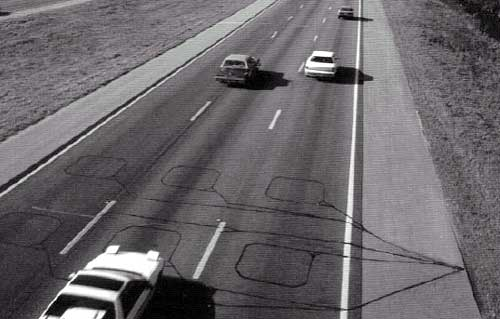
\includegraphics[height=2.5in]{loop_detector.jpg}}

\end{frame}
%%%%%%%%%%%%%%%%%%%%%%%%%%%%%%%%%%%%%%%%%%%%%%%%%%%%%%%%%%%%
\begin{frame}

\frametitle{Caltrans Performance Measurement System (PeMS) records this
data for the whole state}

    \begin{itemize}
        \item Each sensor measures 3 quantities
        \item Every thirty seconds they produce a new data point
        \item $43,680$ sensors in California
        \item $\implies$  377 million new data points per day
    \end{itemize}

\end{frame}
%%%%%%%%%%%%%%%%%%%%%%%%%%%%%%%%%%%%%%%%%%%%%%%%%%%%%%%%%%%%
\begin{frame}

    \frametitle{Traffic engineers study the relationship between 
    density and flow \cite{li2011fundamental}}

\centerline{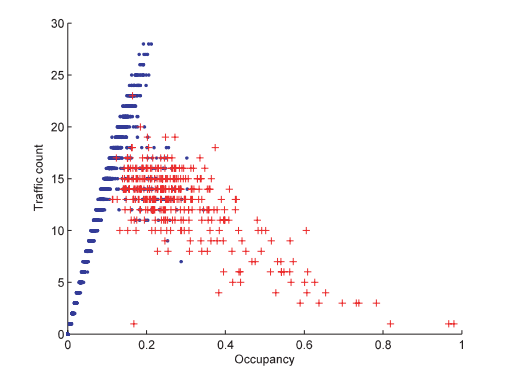
\includegraphics[height=2.5in]{fundamental_diagram.png}}

\end{frame}
%%%%%%%%%%%%%%%%%%%%%%%%%%%%%%%%%%%%%%%%%%%%%%%%%%%%%%%%%%%%
\begin{frame}

    \frametitle{Using more data allows new types of analyses}

    \begin{itemize}
        \item Finding groups of similar detectors
        \item Effect of policy such as speed limits and carpool lanes
        \item Impact of road features such as on/off ramps
        \item Effect of weather
    \end{itemize}

\end{frame}
%%%%%%%%%%%%%%%%%%%%%%%%%%%%%%%%%%%%%%%%%%%%%%%%%%%%%%%%%%%%
\begin{frame}

    \frametitle{Lets scale up the computations with parallel programming}

    \begin{itemize}
        \item Several parallel strategies exist to improve performance
        \item Which is best depends on the platform and data
        \item Each one requires deeper knowledge of that particular technology
        \item Therefore techniques to programmatically identify and use the parallel
  patterns implicit in code would be valuable
    \end{itemize}

\end{frame}
%%%%%%%%%%%%%%%%%%%%%%%%%%%%%%%%%%%%%%%%%%%%%%%%%%%%%%%%%%%%
\section{Simple Example}
%%%%%%%%%%%%%%%%%%%%%%%%%%%%%%%%%%%%%%%%%%%%%%%%%%%%%%%%%%%%
\begin{frame}[fragile]

\frametitle{Illustrate different parallel computational models}

Consider computing the mean,

\begin{equation}
    \bar{x} = \frac{1}{n} \sum_{i = 1}^n x_i
\label{eq:mean}
\end{equation}

where the $x_i$'s are i.i.d. $\sim N(0, 1)$. 
    
In R this code is written:

\begin{verbatim}
xbar = mean(rnorm(n))
\end{verbatim}

\end{frame}
%%%%%%%%%%%%%%%%%%%%%%%%%%%%%%%%%%%%%%%%%%%%%%%%%%%%%%%%%%%%
\begin{frame}

    \frametitle{This can also be expressed as a weighted mean}

\begin{equation}
    \bar{x} = \frac{1}{n} \sum_{j = 1}^p \sum_{i = 1}^{n_j} x_{ij}
    = \sum_{j = 1}^p \frac{n_j}{n} \bar{x}_j
\label{eq:mean_partial}
\end{equation}

Suppose that all $n_i$'s are the same for the following examples.

\end{frame}
%%%%%%%%%%%%%%%%%%%%%%%%%%%%%%%%%%%%%%%%%%%%%%%%%%%%%%%%%%%%
\begin{frame}[fragile]

    \frametitle{The weighted mean can be directly translated into R code}

\begin{verbatim}
meanrnorm = function(n) mean(rnorm(n))

partial_means = sapply(rep(n_i, p), meanrnorm)
xbar = mean(partial_means)
\end{verbatim}

\pause 

    \begin{itemize}
        \item While not parallel, this effectively removes the memory limits.
        \item How to choose the $n_i$ and $p$?
    \end{itemize}

\end{frame}
%%%%%%%%%%%%%%%%%%%%%%%%%%%%%%%%%%%%%%%%%%%%%%%%%%%%%%%%%%%%
\begin{frame}[fragile]

    \frametitle{Send code to workers in a SNOW cluster}

\begin{verbatim}
partial_means = parallel::clusterCall(cluster, meanrnorm, n_i)
\end{verbatim}

\end{frame}
%%%%%%%%%%%%%%%%%%%%%%%%%%%%%%%%%%%%%%%%%%%%%%%%%%%%%%%%%%%%
\begin{frame}[fragile]

    \frametitle{A system \texttt{fork()} can share read only data}

\begin{verbatim}
x = rnorm(n)

starting_indices = as.integer(seq(from = 1, to = n, by = n_i))
ending_indices = starting_indices + (n_i - 1L)

index_mean = function(start, end) mean(x[start:end])

partial_means = parallel::mcmapply(index_mean, starting_indices, ending_indices)
\end{verbatim}

\end{frame}
%%%%%%%%%%%%%%%%%%%%%%%%%%%%%%%%%%%%%%%%%%%%%%%%%%%%%%%%%%%%
\begin{frame}[fragile]

    \frametitle{GPU code can use shared (device) memory}

\begin{verbatim}
# include <random.h>

__kernel void meanrnorm(__global float *x
        , __global float *partial_means
        , int n_i
        )
{
    int id = get_global_id(0);

    Random random_state = seed_rand(id);
    int start_index = id * n_i;
    int end_index = start_index + n_i;

    for(int i = start_index; i < end_index; i++)
    {
        random_state = next_rand(random_state);
        x[i] = rnorm(random_state);
    }
    xbar_local = mean(x, start_index, end_index);
    partial_means[id] = xbar_local;
}
\end{verbatim}

\end{frame}
%%%%%%%%%%%%%%%%%%%%%%%%%%%%%%%%%%%%%%%%%%%%%%%%%%%%%%%%%%%%
\begin{frame}[fragile]

    \frametitle{File backed data structures help with memory and
    parallelism}

\begin{verbatim}
x = bigmemory::filebacked.big.matrix(nrow = n_i, ncol = p, backingfile = "x.bigmatrix")
for (j in seq(p)){
    x[, j] = rnorm(n_i)
}
xbar = biganalytics::mean(x)
\end{verbatim}

% mention interaction effect, using SNOW

\end{frame}
%%%%%%%%%%%%%%%%%%%%%%%%%%%%%%%%%%%%%%%%%%%%%%%%%%%%%%%%%%%%
\begin{frame}[fragile]

    \frametitle{Parallelism can also happen in a pipeline of data
    processing steps}

\begin{verbatim}
# Worker 1
x_chunk = rnorm(n_i)
serialize(x_chunk, worker2)
\end{verbatim}

The second worker receives the random numbers and computes the mean.

\begin{verbatim}
# Worker 2
x_chunk = unserialize(worker1)
partial_means[i] = mean(x_chunk)
i = i + 1
\end{verbatim}

\end{frame}
%%%%%%%%%%%%%%%%%%%%%%%%%%%%%%%%%%%%%%%%%%%%%%%%%%%%%%%%%%%%
\section{Design Considerations}
%%%%%%%%%%%%%%%%%%%%%%%%%%%%%%%%%%%%%%%%%%%%%%%%%%%%%%%%%%%%
\begin{frame}

\frametitle{Different computational models incur their own types of overhead}

    \centerline{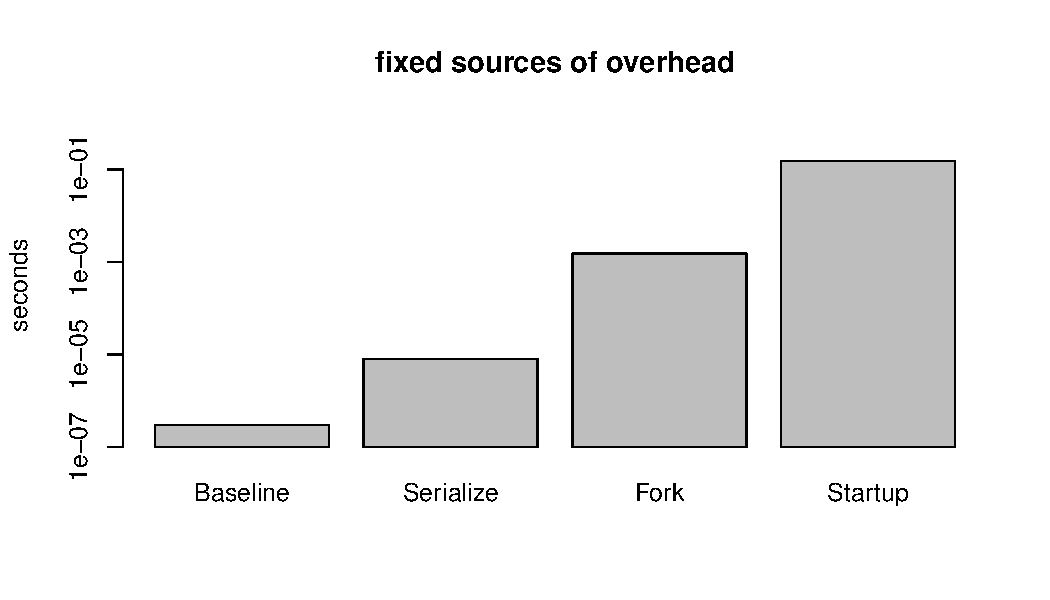
\includegraphics[height=2.5in]{../compute_times/overhead}}

% So if you start up a process, you want to keep it around

\end{frame}
%%%%%%%%%%%%%%%%%%%%%%%%%%%%%%%%%%%%%%%%%%%%%%%%%%%%%%%%%%%%
\begin{frame}

    \frametitle{Layers mark ways for users to write parallel code for one
    platform}

\begin{itemize}
\item User Layer: foreach, future, partools, ddR, biganalytics, RevoScaleR
\item R layer: SNOW, multicore, parallel, bigmemory, Rmpi
\item System Layer: processes, *NIX fork(), memory maps, network sockets,
    MPI
\end{itemize}

\end{frame}
%%%%%%%%%%%%%%%%%%%%%%%%%%%%%%%%%%%%%%%%%%%%%%%%%%%%%%%%%%%%
\begin{frame}

    \frametitle{How can we transform R code into a lower layer?}

\begin{itemize}
    \item \textbf{Plain old R code: \texttt{lapply(), sapply(), for(), \dots}}
\item User Layer: foreach, future, partools, ddR, biganalytics, RevoScaleR
\item R layer: SNOW, multicore, parallel, bigmemory, Rmpi
\item System Layer: processes, *NIX fork(), memory maps, network sockets,
    MPI
\end{itemize}

% Potentially we can transform to any of these layers

\end{frame}
%%%%%%%%%%%%%%%%%%%%%%%%%%%%%%%%%%%%%%%%%%%%%%%%%%%%%%%%%%%%
\section{Code Analysis}
%%%%%%%%%%%%%%%%%%%%%%%%%%%%%%%%%%%%%%%%%%%%%%%%%%%%%%%%%%%%
\begin{frame}

    \frametitle{Apply family of functions / vectorization}

\end{frame}
%%%%%%%%%%%%%%%%%%%%%%%%%%%%%%%%%%%%%%%%%%%%%%%%%%%%%%%%%%%%
\begin{frame}

    \frametitle{Reduce functions}


\end{frame}
%%%%%%%%%%%%%%%%%%%%%%%%%%%%%%%%%%%%%%%%%%%%%%%%%%%%%%%%%%%%
\begin{frame}

    \frametitle{Creating efficient code as a constrained optimization
    problem}



%%%%%%%%%%%%%%%%%%%%%%%%%%%%%%%%%%%%%%%%%%%%%%%%%%%%%%%%%%%%

\begin{frame}[t,allowframebreaks]
\frametitle{References}
\printbibliography
\end{frame}

\end{document}
